%---------------------------------------------------------------------  
    \section{Resultados/Discusión}
    %------------------------------ SLIDE ---------------------------------------
    \begin{frame}{Resultados/Discusión} % cada entorno frame es una diapositiva
        \justifying % para justificar el texto, siempre al inicio de cada frame
        % Añade espacio para mover el bloque hacia arriba
        % Añade espacio para mover el bloque hacia arriba
        \vspace*{-0.4cm} % Ajusta este valor según sea necesario
        
        % Cuadro sin bordes redondeados, con colores personalizados
        \begin{tcolorbox}[colback=custombgcolor3, coltext=customfgcolor2,
                      colframe=custombgcolor3, % Color del borde
                      width=\textwidth,       % Ancho del cuadro
                      boxrule=1pt,            % Grosor del borde
                      top=0.1mm, bottom=0.1mm,     % Espacio superior e inferior
                      sharp corners=all,     % Bordes sin redondear
                      halign=center,         % Alineación horizontal
                      valign=center,         % Alineación vertical
                      ]
            % Texto dentro del cuadro
            %\textbf{Espectro \kern-0.5em de \kern-0.5em partículas \kern-0.5em a \kern-0.5em 7 m.s.n.m.}
            \textbf{Espectro de partículas a 7 m.s.n.m.}        
        \end{tcolorbox}
        \vspace*{-0.4cm} % Ajusta este valor según sea necesario
        
        \begin{figure}
            \centering
            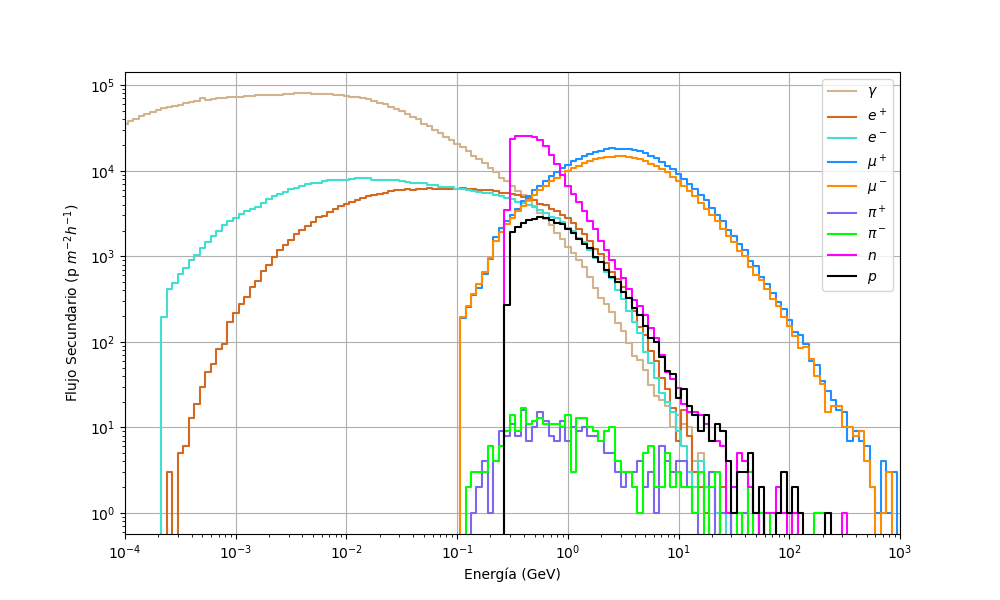
\includegraphics[width=0.74\textwidth]{Figures/Thesis_flux_new2_7msnm_without_title.png}
            \caption{\tiny Espectro de partículas secundarias obtenido a una altura de 7 m s.n.m.  Los colores corresponden a las diferentes partículas secundarias que lograron llegar al nivel de observación.}
        \end{figure}
    \end{frame}     
    
    %------------------------------ SLIDE ---------------------------------------
    \begin{frame}{} % cada entorno frame es una diapositiva
        \justifying % para justificar el texto, siempre al inicio de cada frame
        % Añade espacio para mover el bloque hacia arriba
        % Añade espacio para mover el bloque hacia arriba
        \vspace*{-0.4cm} % Ajusta este valor según sea necesario

        % Cuadro sin bordes redondeados, con colores personalizados
        \begin{tcolorbox}[colback=custombgcolor2, coltext=customfgcolor2,
                      colframe=custombgcolor2, % Color del borde
                      width=\textwidth,       % Ancho del cuadro
                      boxrule=1pt,            % Grosor del borde
                      top=0.1mm, bottom=0.1mm,     % Espacio superior e inferior
                      sharp corners=all,     % Bordes sin redondear
                      halign=center,         % Alineación horizontal
                      valign=center,         % Alineación vertical
                      ]
            % Texto dentro del cuadro
            %\textbf{Espectro \kern-0.5em de \kern-0.5em partículas \kern-0.5em a \kern-0.5em 7 m.s.n.m.}
            \textbf{Espectro de partículas a 4582.5 m.s.n.m.}        
        \end{tcolorbox}
        \vspace*{-0.4cm} % Ajusta este valor según sea necesario
        
        \begin{figure}
            \centering
            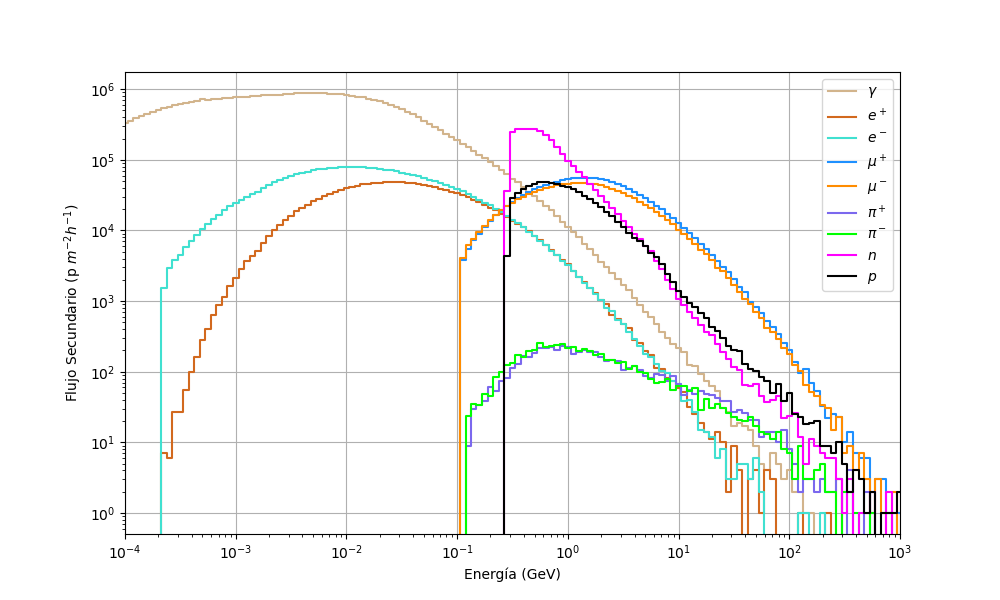
\includegraphics[width=0.82\textwidth]{Figures/Thesis_flux_new2_4600msnm_without_title.png}
            \caption{\tiny Espectro de partículas secundarias obtenido a una altura de 4582.5 m s.n.m. Los colores corresponden a las diferentes partículas secundarias que lograron llegar al nivel de observación.}
        \end{figure}
    \end{frame}

    %------------------------------ SLIDE --------------------------------------- SLIDE DE PRUEBA DE ORIGEN DE RC
    \begin{frame}{} % cada entorno frame es una diapositiva
        \justifying % para justificar el texto, siempre al inicio de cada frame
        % Añade espacio para mover el bloque hacia arriba
        % Añade espacio para mover el bloque hacia arriba
        \vspace*{-0.5cm} % Ajusta este valor según sea necesario
        % Cuadro sin bordes redondeados, con colores personalizados
        
        \begin{columns}
            \begin{column}{0.5\textwidth}
                \centering
                \fcolorbox{black}{custombgcolor3}{
                    \parbox[c][0.5cm][c]{0.8\textwidth}{
                        \centering
                        \footnotesize \textbf{Espectro de partículas a 7 m.s.n.m.}
                    }
                }

                \vspace*{-0.3cm} % Ajusta este valor según sea necesario
                \begin{figure}
                    \centering
				    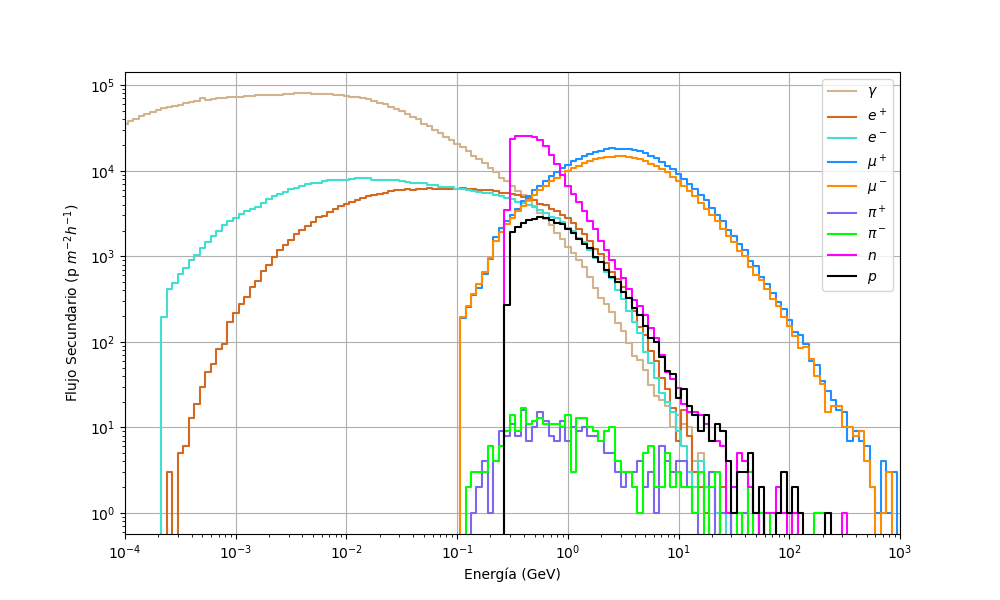
\includegraphics[width=1.13\textwidth]{Figures/Thesis_flux_new2_7msnm_without_title.png}
                \end{figure}
                
            \end{column}

            \begin{column}{0.5\textwidth}
                \centering
                \fcolorbox{black}{custombgcolor2}{
                    \parbox[c][0.5cm][c]{0.8\textwidth}{
                        \centering
                        \footnotesize \textbf{Espectro de partículas a 4582.5 m.s.n.m.}
                    }
                }

                \vspace*{-0.3cm} % Ajusta este valor según sea necesario
                \begin{figure}
                    \centering
				    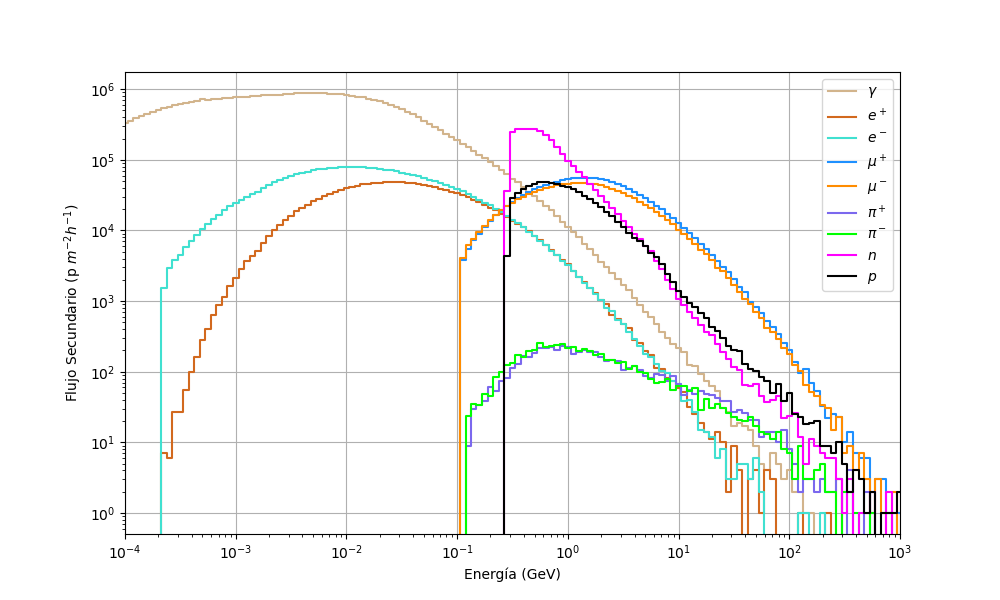
\includegraphics[width=1.13\textwidth]{Figures/Thesis_flux_new2_4600msnm_without_title.png}
                \end{figure}            
            \end{column}
        \end{columns}
    \end{frame}  

    %------------------------------ SLIDE ---------------------------------------
    \begin{frame}{} % cada entorno frame es una diapositiva
        \justifying % para justificar el texto, siempre al inicio de cada frame
        % Añade espacio para mover el bloque hacia arriba
        % Añade espacio para mover el bloque hacia arriba
        \vspace*{-0.3cm} % Ajusta este valor según sea necesario

        % Cuadro sin bordes redondeados, con colores personalizados
        \begin{tcolorbox}[colback=custombgcolor4, coltext=customfgcolor2,
                      colframe=custombgcolor4, % Color del borde
                      width=\textwidth,       % Ancho del cuadro
                      boxrule=1pt,            % Grosor del borde
                      top=0.1mm, bottom=0.1mm,     % Espacio superior e inferior
                      sharp corners=all,     % Bordes sin redondear
                      halign=center,         % Alineación horizontal
                      valign=center,         % Alineación vertical
                      ]
            % Texto dentro del cuadro
            %\textbf{Espectro \kern-0.5em de \kern-0.5em partículas \kern-0.5em a \kern-0.5em 7 m.s.n.m.}
            \textbf{Flujo de neutrones con EXPACS}        
        \end{tcolorbox}
        \vspace*{-0.4cm} % Ajusta este valor según sea necesario
        
        \begin{figure}
            \centering
            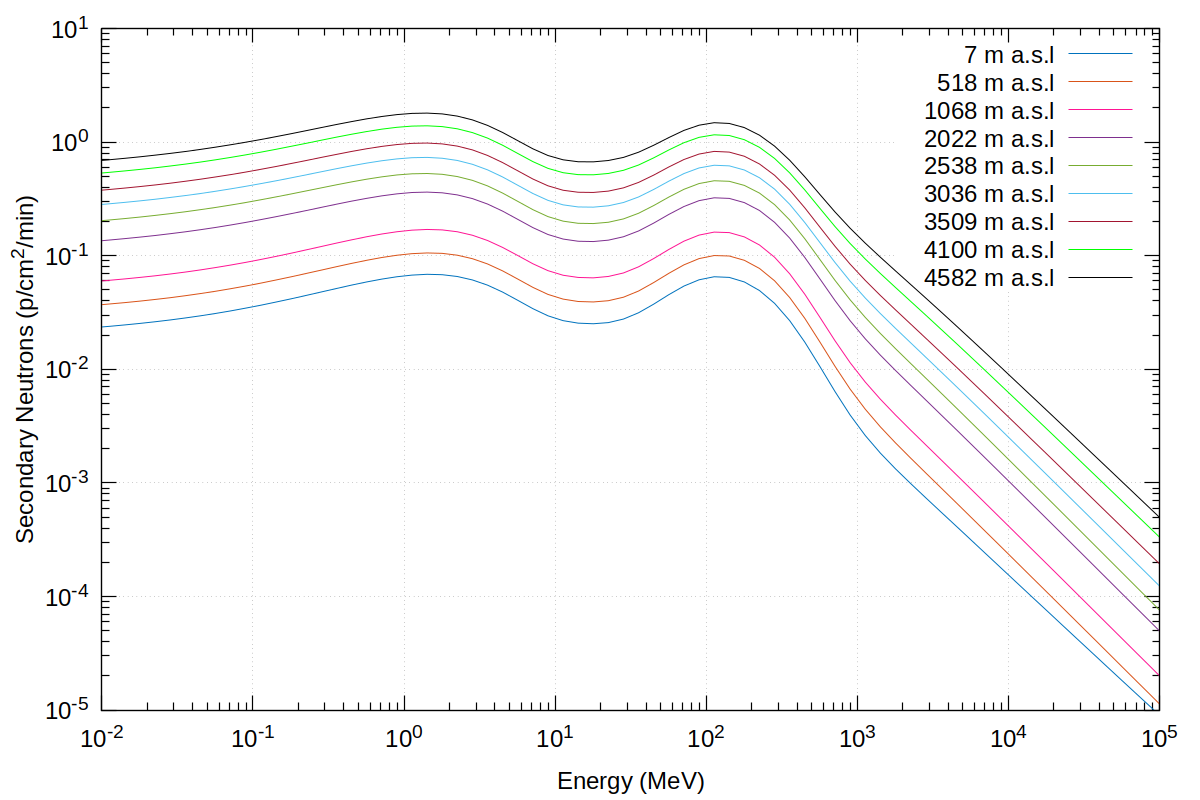
\includegraphics[width=0.75\textwidth]{Figures/Neutron_flux.png}
            \caption{\tiny Espectro de neutrones a diferentes alturas utilizando EXPACS [\cite{sedrati2022}].}
        \end{figure}
    \end{frame}

    %------------------------------ SLIDE ---------------------------------------
    \begin{frame}{} % cada entorno frame es una diapositiva
        \justifying % para justificar el texto, siempre al inicio de cada frame
        % Añade espacio para mover el bloque hacia arriba
        % Añade espacio para mover el bloque hacia arriba
        \vspace*{-0.3cm} % Ajusta este valor según sea necesario

        % Cuadro sin bordes redondeados, con colores personalizados
        \begin{tcolorbox}[colback=custombgcolor8, coltext=customfgcolor2,
                      colframe=custombgcolor8, % Color del borde
                      width=\textwidth,       % Ancho del cuadro
                      boxrule=1pt,            % Grosor del borde
                      top=0.1mm, bottom=0.1mm,     % Espacio superior e inferior
                      sharp corners=all,     % Bordes sin redondear
                      halign=center,         % Alineación horizontal
                      valign=center,         % Alineación vertical
                      ]
            % Texto dentro del cuadro
            %\textbf{Espectro \kern-0.5em de \kern-0.5em partículas \kern-0.5em a \kern-0.5em 7 m.s.n.m.}
            \textbf{Flujo de protones y neutrones vs Altura}        
        \end{tcolorbox}
        \vspace*{-0.4cm} % Ajusta este valor según sea necesario
        
        \begin{figure}
            \centering
            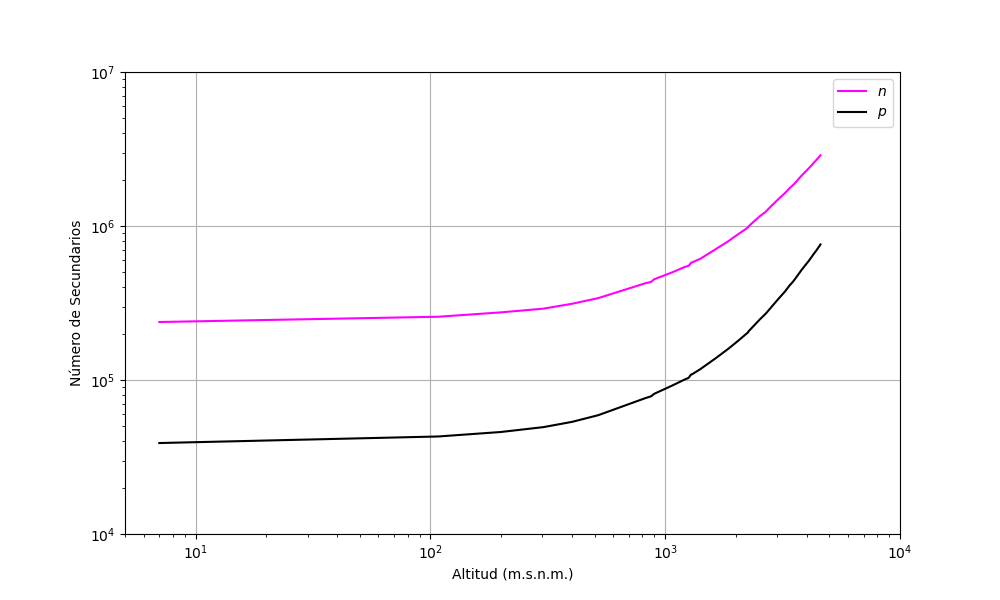
\includegraphics[width=0.81\textwidth]{Figures/Thesis_flux_protons_and_neutrons.png}
            \caption{\tiny Flujo total de protones (negro) y neutrones (rosa) desde nivel del mar hasta cima del volcán Sierra Negra ($4582$.5 m s.n.m.) obtenido a través de las simulaciones con CORSIKA.}
        \end{figure}
    \end{frame} 
    
    %------------------------------ SLIDE ---------------------------------------
    \begin{frame}{} % cada entorno frame es una diapositiva
        \justifying % para justificar el texto, siempre al inicio de cada frame
        % Añade espacio para mover el bloque hacia arriba
        % Añade espacio para mover el bloque hacia arriba
        \vspace*{-0.3cm} % Ajusta este valor según sea necesario

        % Cuadro sin bordes redondeados, con colores personalizados
        \begin{tcolorbox}[colback=custombgcolor9, coltext=customfgcolor2,
                      colframe=custombgcolor9, % Color del borde
                      width=\textwidth,       % Ancho del cuadro
                      boxrule=1pt,            % Grosor del borde
                      top=0.1mm, bottom=0.1mm,     % Espacio superior e inferior
                      sharp corners=all,     % Bordes sin redondear
                      halign=center,         % Alineación horizontal
                      valign=center,         % Alineación vertical
                      ]
            % Texto dentro del cuadro
            %\textbf{Espectro \kern-0.5em de \kern-0.5em partículas \kern-0.5em a \kern-0.5em 7 m.s.n.m.}
            \textbf{Número de cuentas registrado con el MMN}        
        \end{tcolorbox}
        \vspace*{-0.3cm} % Ajusta este valor según sea necesario
        
        \begin{figure}
            \centering
            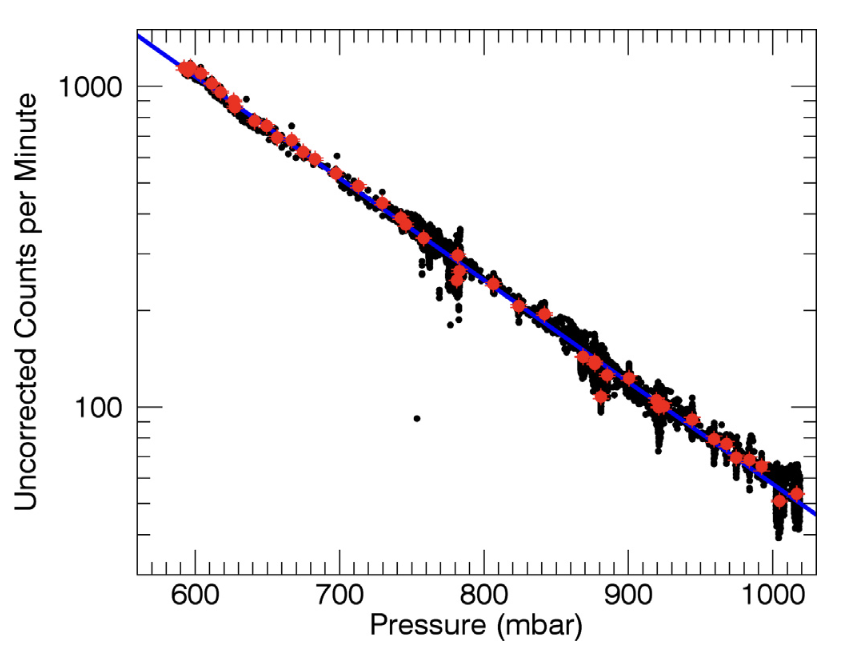
\includegraphics[width=0.6\textwidth]{Figures/rate-MMN.png}
            \caption{\tiny Número de cuentas por minuto en función de la presión observada registrada por el MMN. Los puntos negros representan la tasa media de conteo durante todo el estudio (incluidos los periodos de tiempo cuando se movía el MMN de un punto de observación a otro). Los puntos rojos representan la tasa media de conteo en los puntos de observación [\cite{lara2016}].}
        \end{figure}
    \end{frame}    